\documentclass[
11pt, % The default document font size, options: 10pt, 11pt, 12pt
% codirector, % Uncomment to add a codirector to the title page
]{charter} 


% El títulos de la memoria, se usa en la carátula y se puede usar el cualquier lugar del documento con el comando \ttitle
\titulo{Detección de peso de pollos en fincas broiler} 

% Nombre del posgrado, se usa en la carátula y se puede usar el cualquier lugar del documento con el comando \degreename
%\posgrado{Carrera de Especialización en Sistemas Embebidos} 
%\posgrado{Carrera de Especialización en Internet de las Cosas} 
\posgrado{Carrera de Especialización en Inteligencia Artificial}
%\posgrado{Maestría en Sistemas Embebidos} 
%\posgrado{Maestría en Internet de las cosas}
% IMPORTANTE: no omitir titulaciones ni tildación en los nombres, también se recomienda escribir los nombres completos (tal cual los tienen en su documento)
% Tu nombre, se puede usar el cualquier lugar del documento con el comando \authorname
\autor{Ing. Nicolás Martín Tertusio Iglesias}

% El nombre del director y co-director, se puede usar el cualquier lugar del documento con el comando \supname y \cosupname y \pertesupname y \pertecosupname
\director{Ing. Maxim Dorogov}
\pertenenciaDirector{FIUBA} 
\codirector{} % para que aparezca en la portada se debe descomentar la opción codirector en los parámetros de documentclass
\pertenenciaCoDirector{FIUBA}

% Nombre del cliente, quien va a aprobar los resultados del proyecto, se puede usar con el comando \clientename y \empclientename
\cliente{Ing. Marylin Melo de Simons}
\empresaCliente{Empresas Melo S.A.}
 
\fechaINICIO{19 de junio de 2024}		%Fecha de inicio de la cursada de GdP \fechaInicioName
\fechaFINALPlan{17 de agosto de 2024} 	%Fecha de final de cursada de GdP
\fechaFINALTrabajo{20 de diciembre de 2024}	%Fecha de defensa pública del trabajo final


\begin{document}

\maketitle
\thispagestyle{empty}
\pagebreak

\thispagestyle{empty}
{\setlength{\parskip}{0pt}
\tableofcontents{}
}
\pagebreak


\section*{Registros de cambios}
\label{sec:registro}


\begin{table}[ht]
\label{tab:registro}
\centering
\begin{tabularx}{\linewidth}{@{}|c|X|c|@{}}
\hline
\rowcolor[HTML]{C0C0C0} 
Revisión & \multicolumn{1}{c|}{\cellcolor[HTML]{C0C0C0}Detalles de los cambios realizados} & Fecha      \\ \hline
0      & Creación del documento                                 &\fechaInicioName \\ \hline
1      & Se completa hasta el punto 5 inclusive                 & {26} de {junio} de 2024 \\ \hline
2      & Se completa hasta el punto 9 inclusive                 & {4} de {julio} de 2024 \\ \hline
%		  Se puede agregar algo más \newline
%		  En distintas líneas \newline
%		  Así                                                    & {día} de {mes} de 202X \\ \hline
%3      & Se completa hasta el punto 12 inclusive                & {día} de {mes} de 202X \\ \hline
%4      & Se completa el plan	                                 & {día} de {mes} de 202X \\ \hline

% Si hay más correcciones pasada la versión 4 también se deben especificar acá

\end{tabularx}
\end{table}

\pagebreak



\section*{Acta de constitución del proyecto}
\label{sec:acta}

\begin{flushright}
Panamá, \fechaInicioName
\end{flushright}

\vspace{2cm}

Por medio de la presente se acuerda con el \authorname\hspace{1px} que su Trabajo Final de la \degreename\hspace{1px} se titulará ``\ttitle'' y consistirá en la implementación de un sistema de detección de pesos de pollos en finca broiler por medio de \textit{computer vision} (CV). El trabajo tendrá un presupuesto preliminar estimado de 600 horas y un costo estimado de \$ 10,000.00, con fecha de inicio el \fechaInicioName\hspace{1px} y fecha de presentación pública el \fechaFinalName.

Se adjunta a esta acta la planificación inicial.

\vfill

% Esta parte se construye sola con la información que hayan cargado en el preámbulo del documento y no debe modificarla
\begin{table}[ht]
\centering
\begin{tabular}{ccc}
\begin{tabular}[c]{@{}c@{}}Dr. Ing. Ariel Lutenberg \\ Director posgrado FIUBA\end{tabular} & \hspace{2cm} & \begin{tabular}[c]{@{}c@{}}\clientename \\ \empclientename \end{tabular} \vspace{2.5cm} \\ 
\multicolumn{3}{c}{\begin{tabular}[c]{@{}c@{}} \supname \\ Director del Trabajo Final\end{tabular}} \vspace{2.5cm} \\
\end{tabular}
\end{table}




\section{1. Descripción técnica-conceptual del proyecto a realizar}
\label{sec:descripcion}

% El bloque "consigna" se usa para poner texto en rojo y dar una pequeña ayuda sobre cómo completar la sección. En cada entrega parcial deben eliminar los comandos begin y end del bloque consigna de las secciones que hayan completado.
Empresas Melo S.A. es una empresa de Panamá con una integración vertical en la industria avícola. La compañía se encarga de todo el proceso productivo, desde la creación de alimentos para pollos a partir de materia prima, pasando por la crianza de pollos tipo broiler (de engorde), gallinas ponedoras de huevo y pollos para reproducción, hasta llegar a una planta de sacrificio donde se procesan los pollos según la demanda. Finalmente, los productos pueden ser enviados a una planta de valor agregado donde se crean artículos como milanesas, nuggets, entre otros.

El proyecto se enfoca en el segundo paso: la crianza de los pollos broiler. En las fincas, los pollos se crían en espacios, denominados fincas, que pueden albergar hasta 40.000 aves en 950 m². Actualmente, el peso de los pollos se determina mediante muestreos semanales de 100 a 300 ejemplos, lo que representa menos del 1\% del total, un método que no cumple con los estándares precisos exigidos por el mercado. Para resolver este problema, se propone la instalación de cámaras especializadas en \textit{computer vision} (CV) dentro de las fincas. Estas cámaras capturan imágenes de los pollos y mediante modelos de inteligencia artificial (IA) determinan el peso de cada ave.

En la figura \ref{fig:diagBloques} se presenta el diagrama en bloques del sistema. El proceso comienza con las cámaras de video, que inician la detección de peso mediante el preprocesamiento de las imágenes. Estas imágenes se envían al primer modelo de segmentación y clasificación, cuyo resultado son recortes individuales de cada pollo detectado. A continuación, estos recortes alimentan el segundo modelo de predicción de peso, del cual se obtiene el peso individual de cada ave. Con esta información se calcula el peso promedio de los pollos en la finca y se determina la distribución de los mismos. Los resultados se envían a un sistema de monitoreo y reporte, que junto con la transmisión de video, es accesible para el personal de la finca. Esto permite supervisar el estado de los pollos y determinar el momento adecuado para enviarlos a la planta de sacrificio.

\begin{figure}[htpb]
\centering 
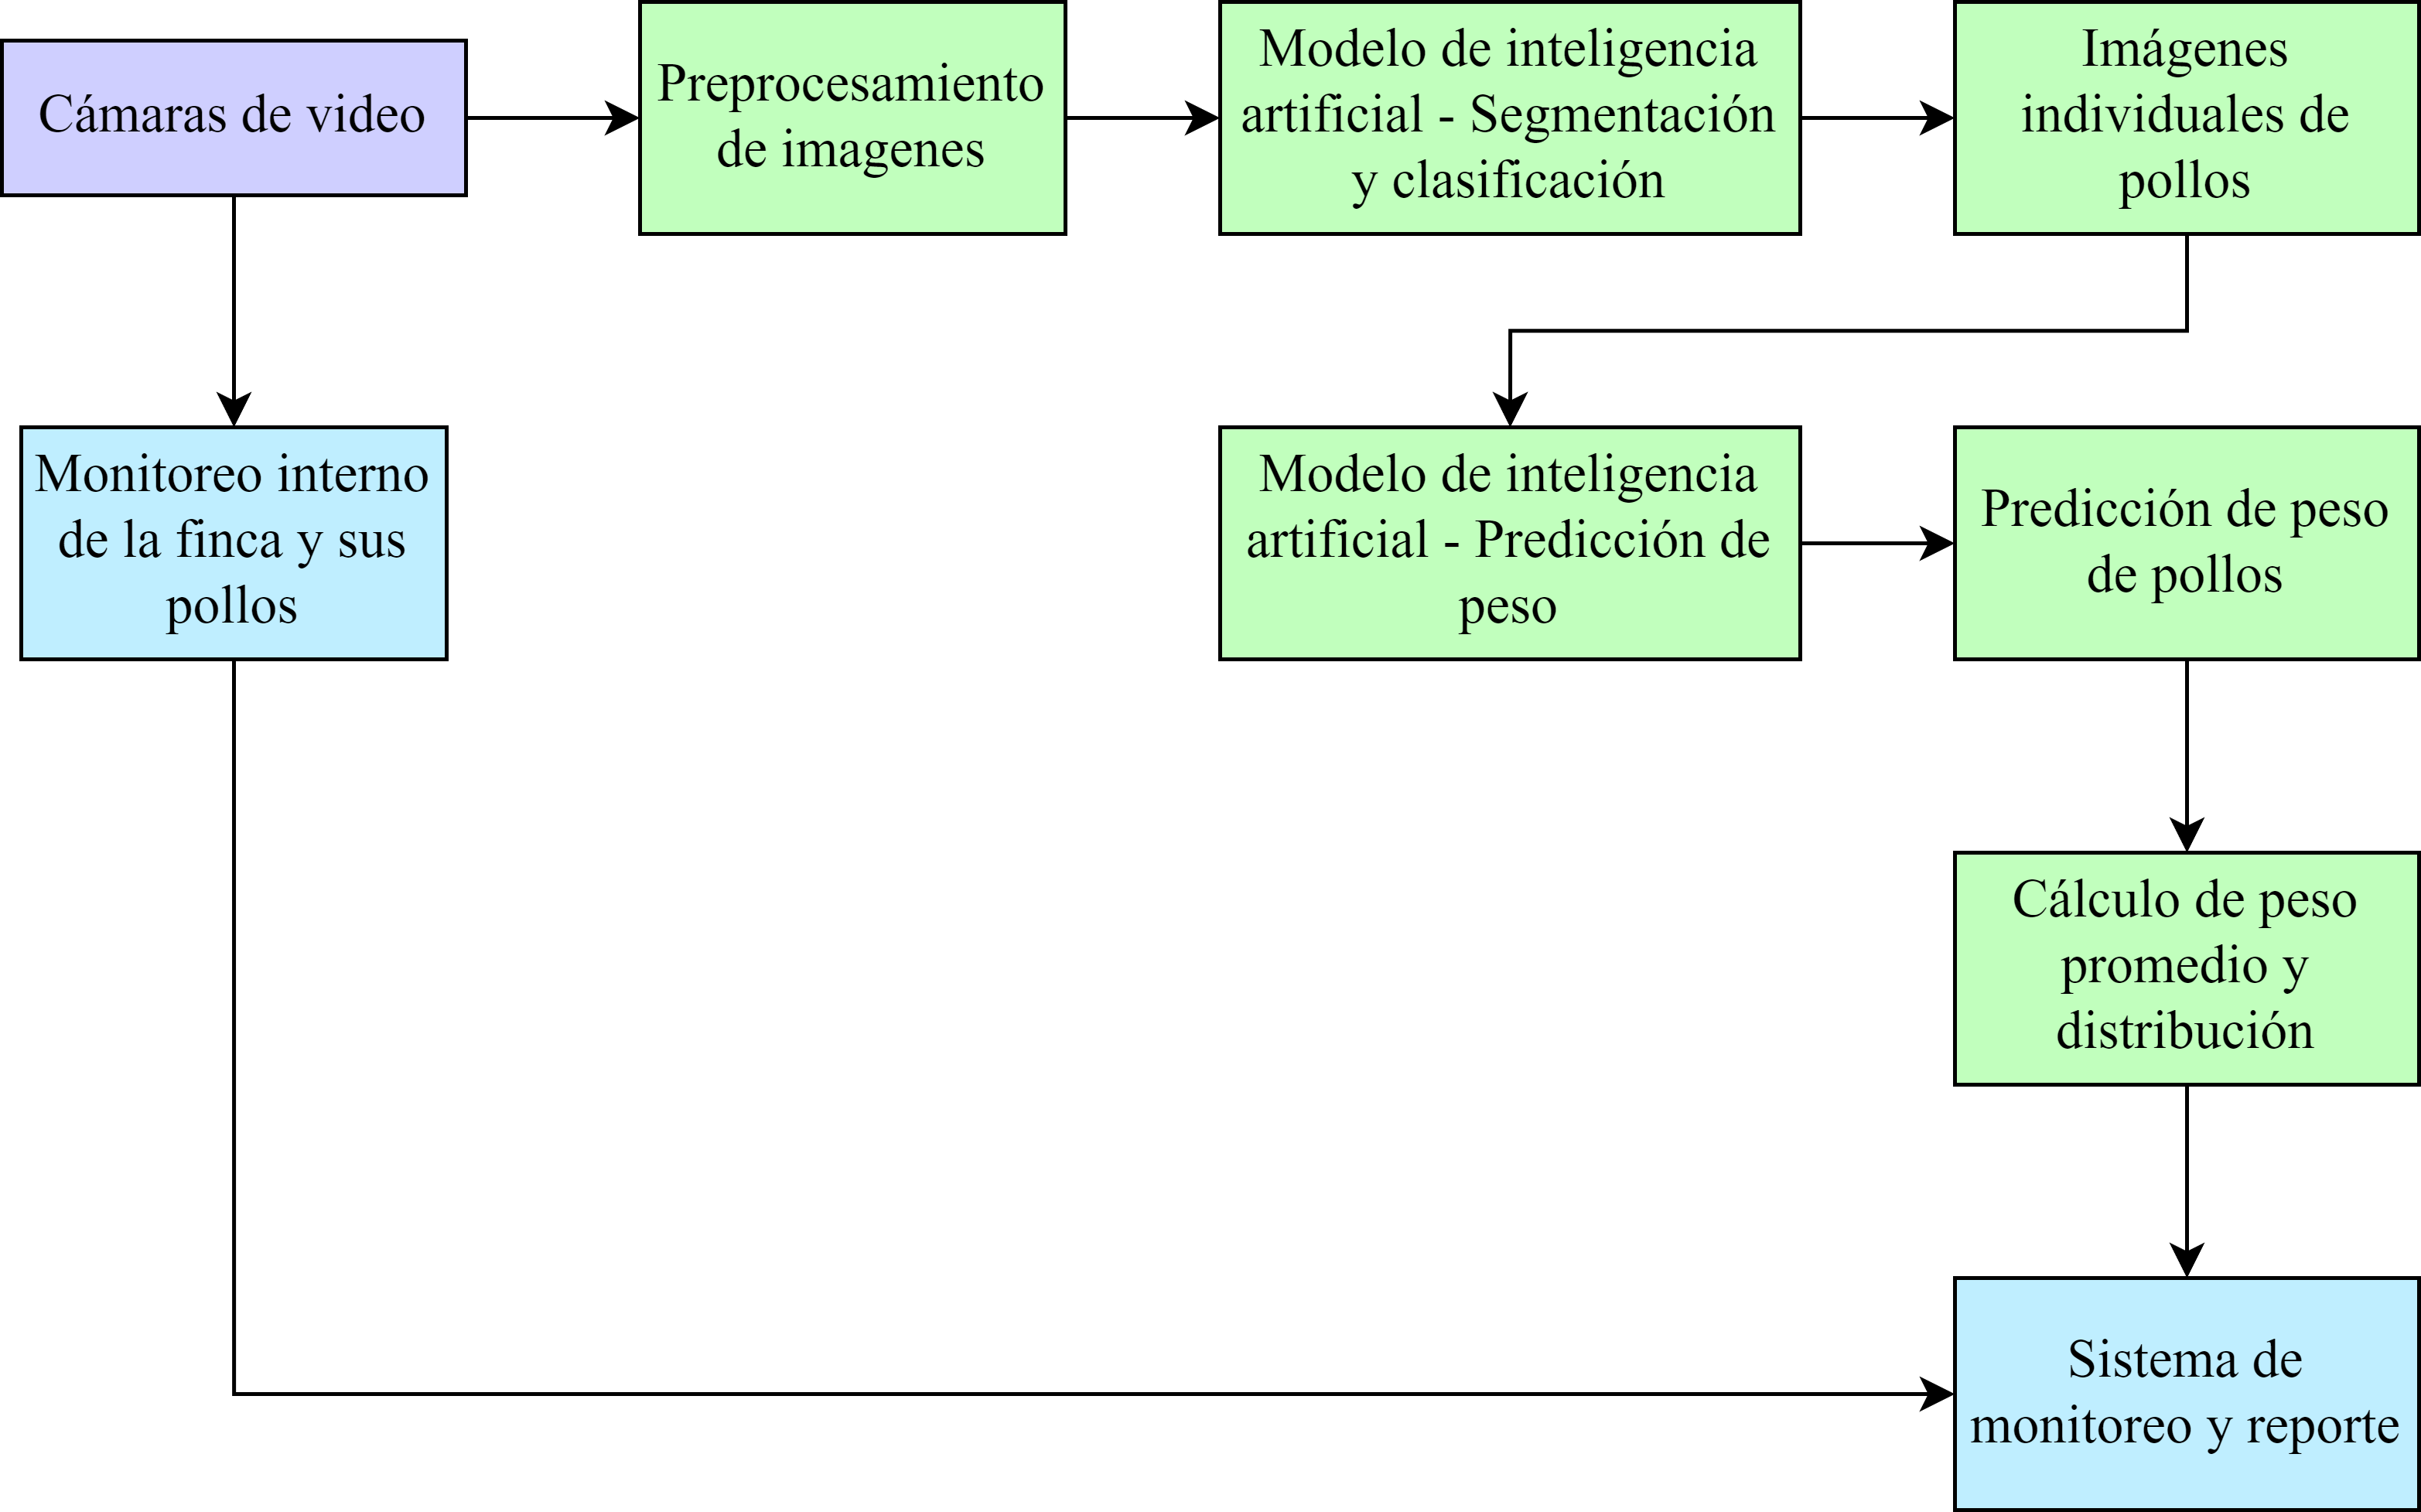
\includegraphics[width=.85\textwidth]{./Figuras/diagBloques2.png}
\caption{Diagrama en bloques del sistema.}
\label{fig:diagBloques}
\end{figure}

\vspace{25px}

\section{2. Identificación y análisis de los interesados}
\label{sec:interesados}

\begin{table}[ht]
%\caption{Identificación de los interesados}
%\label{tab:interesados}
\begin{tabularx}{\linewidth}{@{}|l|X|X|X|@{}}
\hline
\rowcolor[HTML]{C0C0C0} 
Rol           & Nombre y Apellido & Organización 	& Puesto 	\\ \hline
%Auspiciante   &                   &              	&        	\\ \hline
Cliente       & \clientename      &\empclientename	& Directora de operaciones (COO)	\\ \hline
%Impulsor      &                   &              	&        	\\ \hline
Responsable   & \authorname       & FIUBA        	& Alumno 	\\ \hline
Colaboradores & Kelvin Vega       &\empclientename   & Mantenimiento de fincas       	\\ \hline
Orientador    & \supname	      & \pertesupname 	& Director del Trabajo Final \\ \hline
%Equipo        & miembro1 \newline 
%				miembro2          &              	&        	\\ \hline
%Opositores    &                   &              	&        	\\ \hline
Usuario final & Diógenes Becerra         &\empclientename	& Vicepresidente de división Producción       	\\ \hline
\end{tabularx}
\end{table}

\begin{itemize}
	\item Usuario final: se coloca al vicepresidente porque cumple con la figura de representar la división. Sin embargo, los usuarios finales son todo el personal operativo de la finca.
\end{itemize}

\section{3. Propósito del proyecto}
\label{sec:proposito}
El propósito de este proyecto es desarrollar un sistema de monitoreo mediante cámaras de video instaladas en una finca, capaz de predecir el peso de los pollos utilizando técnicas de IA y VC. Este sistema ofrecerá una distribución de peso más precisa que el método de muestreo actual, eliminará el proceso manual de muestreo, permitirá conocer el momento exacto en el que se puede llevar la parvada a la planta de sacrificio y reducirá el consumo de alimento y agua de los pollos.

\section{4. Alcance del proyecto}
\label{sec:alcance}
El proyecto contempla la parte de hardware y software a desarrollar para el diagrama en bloques especificado en la figura \ref{fig:diagBloques}. A desarrollar por el estudiante están las siguientes tareas:

\begin{itemize}
\item Recibir las imágenes de las cámaras de video para iniciar el pipeline de preprocesamiento de las mismas.
\item Implementación de un modelo que, por medio de técnicas de IA y CV, pueda distinguir por lo menos un 80\% de los pollos que se encuentren presentes en una foto.
	\begin{itemize}
	\item Obtención de imágenes para el entrenamiento del modelo seleccionado.
	\item Etiquetado de las imágenes para permitir aprendizaje supervisado.
	\end{itemize}
\item Preprocesamiento de las imágenes de salida del modelo anteriormente mencionado.
\item Implementación de un modelo de IA capaz de predecir, por medio de características físicas y visuales de las aves, el peso de las mismas.
	\begin{itemize}
	\item Al igual que para el primer modelo, se incluye la obtención de imágenes y etiquetado de las mismas.
	\end{itemize}
\item Desarrollo estadístico sobre la distribución de pesos de la parvada.
\item Creación de una interfaz que muestre a los usuarios finales la distribución y peso promedio de los pollos dentro de la finca.
\end{itemize}

A pesar de que está incluido en el alcance del proyecto, no será desarrollado por el estudiante la instalación de cámaras de video. Esto será tercerizado por \empclientename

\section{5. Supuestos del proyecto}
\label{sec:supuestos}
Para el desarrollo del presente proyecto se supone que:

\begin{itemize}
	\item Se dispone de 16 horas semanales para el desarrollo del mismo.
	\item Se tendrá acceso a un stream continuo de video de todas las cámaras instaladas dentro de la finca. 
	\item Se cuenta con una computadora con capacidad computacional suficiente, o un servicio tercerizado similar, para el entrenamiento de los modelos de IA.
	\item Se tendrá disponibilidad limitada para ingresar a la finca y realizar trabajos dentro de la misma, dependiendo de la ocupación de la misma y la naturaleza de los trabajos a realizar.
	\item Se acepta una precisión dentro de un margen razonable de $\pm$10\% para la predicción de pesos de las aves. 
\end{itemize}

\section{6. Requerimientos}
\label{sec:requerimientos}

\begin{enumerate}
	\item Requerimientos de entrenamiento
		\begin{enumerate}
		\item Se deberá instalar cámaras de video dentro de la finca.
		\item Se deberá levantar la información de entrenamiento de los modelos desde cero y etiquetarla.
		\end{enumerate}
	\item Requerimientos funcionales
		\begin{enumerate}
		\item El sistema será capaz de identificar a la mayoría de pollos que aparece en cada cámara de video.
		\item El sistema será capaz de segmentar por medio de coordenadas cada una de las aves.
		\item El sistema será capaz de detectar características visuales de cada pollo.
		\item El sistema será capaz de predecir un peso a cada imagen de ave que identifique.
		\end{enumerate}
	\item Requerimientos de documentación
		\begin{enumerate}
		\item Se deberá elaborar una memoria técnica para el proyecto.
		\item Se deberá documentar todo el procesamiento de imágenes que se realice.
		\item El proyecto deberá tener un control de versiones por medio de un repositorio de GitHub o similar para mantener un control de versiones.
		\end{enumerate}
	\item Requerimiento de desempeño
		\begin{enumerate}
		\item El procesamiento de video y las detecciones será en tiempo real.
		\item El sistema será capaz de predecir con un margen de $\pm$10\% el peso de cada pollo.
		\end{enumerate}
	\item Requerimientos de la interfaz
		\begin{enumerate}
		\item La interfaz deberá mostrar la distribución de pesos de los pollos.
		\item La interfaz deberá mostrar el peso promedio estimado de la parvada.
		\item La interfaz deberá mostrar el peso promedio de la parvada a lo largo del tiempo.
		\item Se deberá poder interactuar con la interfaz para dar inicio a un nuevo lote de pollos.
		\end{enumerate}
\end{enumerate}

\section{7. Historias de usuarios (\textit{Product backlog})}
\label{sec:backlog}

Descripción: en esta sección se deben incluir las historias de usuarios y su ponderación (\textit{history points}). Recordar que las historias de usuarios son descripciones cortas y simples de una característica contada desde la perspectiva de la persona que desea la nueva capacidad, generalmente un usuario o cliente del sistema. La ponderación es un número entero que representa el tamaño de la historia comparada con otras historias de similar tipo.

Se debe indicar explícitamente el criterio para calcular los \textit{story points} de cada historia.

El formato propuesto es: 
\begin{enumerate}
\item Como gerente de producción, quiero ver la evolución del peso promedio de la parvada a lo largo del tiempo en la interfaz, para detectar tendencias y hacer ajustes en la crianza.

\textit{Story points}: 5 (complejidad: 2, dificultad: 2, incertidumbre: 1)
\item Como supervisor de la finca, quiero interactuar con la interfaz del sistema para iniciar un nuevo lote de pollos, para asegurar un manejo ordenado y documentado de cada ciclo de producción.

\textit{Story points}: 3 (complejidad: 1, dificultad: 1, incertidumbre: 1)
\item Como trabajador de la finca, quiero que el sistema prediga el peso de cada pollo basado en las imágenes, para tomar decisiones informadas sobre el momento adecuado para llevar las aves a la planta de sacrificio.

\textit{Story points}: 13 (complejidad: 5, dificultad: 4, incertidumbre: 3)
\item Como gerente de operaciones, quiero que se guarde la información al iniciar un lote nuevo, para llevar un histórico de parvadas anteriores.

\textit{Story points}: 13 (complejidad: 3, dificultad: 2, incertidumbre: 4)
\end{enumerate}

\section{8. Entregables principales del proyecto}
\label{sec:entregables}

Los entregables del proyecto son (ejemplo):

\begin{itemize}
	\item Manual de usuario.
	\item Código fuente del firmware.
	\item Interfaz web para ver el peso promedio, cambio en el tiempo de la misma y distribución de pesos actual.
	\item Memoria del trabajo final.
\end{itemize}

\section{9. Desglose del trabajo en tareas}
\label{sec:wbs}

\begin{enumerate}
\item Compra de equipos (35 horas)
	\begin{enumerate}
	\item Comprar las cámaras de video a utilizar e instalarlas dentro de la finca. (32 horas)
	\item Comprar un ordenador o contratar un servicio en la nube para el entrenamiento de los modelos de IA. (asíncrono, 3 horas)
	\end{enumerate}
\item Toma de datos (170 horas)
	\begin{enumerate}
	\item Capturar imágenes de pollos en diferentes condiciones de iluminación y ángulos. (75 horas)
	\item Asegurar una cantidad suficiente de imágenes para una segmentación robusta. (10 horas)
	\item Capturar imágenes de pollos junto con mediciones precisas de su peso. (75 horas)
	\item Garantizar variedad en el tamaño y peso de los pollos en las imágenes. (10 horas)
	\end{enumerate}
\item Etiquetado de datos (30 horas)
	\begin{enumerate}
	\item Utilizar software de etiquetado para marcar y clasificar cada pollo en las imágenes. (15 horas)
	\item Asociar cada imagen con el peso real del pollo. (15 horas)
	\end{enumerate}
\item Desarrollo del pipeline de preprocesamiento (30 horas)
	\begin{enumerate}
	\item Escribir códigos para limpiar y preparar las imágenes. (20 horas)
	\item Aplicar técnicas de aumento de datos para mejorar la robustez del modelo. (10 horas)
	\end{enumerate}
\item Entrenamiento del modelo de segmentación y clasificación (120 horas)
	\begin{enumerate}
	\item Seleccionar y configurar el modelo de IA apropiado. (20 horas)
	\item Entrenar el modelo utilizando las imágenes etiquetadas. (100 horas)
	\end{enumerate}
\item Entrenamiento del modelo de predicción de peso (75 horas)
	\begin{enumerate}
	\item Seleccionar y configurar el modelo de IA apropiado. (15 horas)
	\item Entrenar el modelo utilizando las imágenes etiquetadas con peso. (60 horas)
	\end{enumerate}
\item Desarrollo de la interfaz web (75 horas)
	\begin{enumerate}
	\item Desarrollar la interfaz utilizando tecnologías web (como HTML y CSS). (15 horas)
	\item Integrar el \textit{backend} para mostrar datos en tiempo real. (25 horas)
	\item Implementar gráficos para mostrar el peso promedio. (5 horas)
	\item Implementar gráficos históricos para mostrar la evolución del peso. (5 horas)
	\item Desarrollar funcionalidad para iniciar y gestionar nuevos lotes de pollos. (5 horas)
	\item Realizar pruebas de usabilidad con los usuarios finales. (20 horas)
	\end{enumerate}
\item Documentación (65 horas)
	\begin{enumerate}
	\item Documentar el etiquetado y preprocesamiento de imágenes. (15 horas)
	\item Documentar el entrenamiento y evaluación de los modelos de IA. (35 horas)
	\item Documentar el desarrollo e implementación de la interfaz web. (15 horas)
	\end{enumerate}
\end{enumerate}

Cantidad total de horas: 600 horas.

\section{10. Diagrama de Activity On Node}
\label{sec:AoN}

\begin{consigna}{red}
Armar el AoN a partir del WBS definido en la etapa anterior.

Una herramienta simple para desarrollar los diagramas es el Draw.io (\url{https://app.diagrams.net/}).
\href{https://app.diagrams.net}{Draw.io}


\begin{figure}[htpb]
\centering 
\includegraphics[width=.8\textwidth]{./Figuras/AoN.png}
\caption{Diagrama de \textit{Activity on Node}.}
\label{fig:AoN}
\end{figure}

Indicar claramente en qué unidades están expresados los tiempos.
De ser necesario indicar los caminos semi críticos y analizar sus tiempos mediante un cuadro.
Es recomendable usar colores y un cuadro indicativo describiendo qué representa cada color.

\end{consigna}

\section{11. Diagrama de Gantt}
\label{sec:gantt}

\begin{consigna}{red}
Existen muchos programas y recursos \textit{online} para hacer diagramas de Gantt, entre los cuales destacamos:

\begin{itemize}
\item Planner
\item GanttProject
\item Trello + \textit{plugins}. En el siguiente link hay un tutorial oficial: \\ \url{https://blog.trello.com/es/diagrama-de-gantt-de-un-proyecto}
\item Creately, herramienta online colaborativa. \\\url{https://creately.com/diagram/example/ieb3p3ml/LaTeX}
\item Se puede hacer en latex con el paquete \textit{pgfgantt}\\ \url{http://ctan.dcc.uchile.cl/graphics/pgf/contrib/pgfgantt/pgfgantt.pdf}
\end{itemize}

Pegar acá una captura de pantalla del diagrama de Gantt, cuidando que la letra sea suficientemente grande como para ser legible. 
Si el diagrama queda demasiado ancho, se puede pegar primero la ``tabla'' del Gantt y luego pegar la parte del diagrama de barras del diagrama de Gantt.

Configurar el software para que en la parte de la tabla muestre los códigos del EDT (WBS).\\
Configurar el software para que al lado de cada barra muestre el nombre de cada tarea.\\
Revisar que la fecha de finalización coincida con lo indicado en el Acta Constitutiva.

En la figura \ref{fig:gantt}, se muestra un ejemplo de diagrama de gantt realizado con el paquete de \textit{pgfgantt}. 
En la plantilla pueden ver el código que lo genera y usarlo de base para construir el propio.

Las fechas pueden ser calculadas utilizando alguna de las herramientas antes citadas. Sin embargo, el siguiente ejemplo
fue elaborado utilizando 
\href{https://docs.google.com/spreadsheets/d/1fBz8NhSpc4tkkhz3KjJCbh1nR_ltDkfEcZi4tZXduqs}{esta hoja de cálculo}.

Es importante destacar que el ancho del diagrama estará dado por la longitud del texto utilizado para las tareas 
(Ejemplo: tarea 1, tarea 2, etcétera) y el valor \textit{x unit}. Para mejorar la apariencia del diagrama, es necesario
ajustar este valor y, quizás, acortar los nombres de las tareas.

\begin{figure}[htpb]
  \begin{center}
    \begin{ganttchart}[
      time slot unit=day,
      time slot format=isodate,
      x unit=0.038cm,
      y unit title=0.7cm,
      y unit chart=0.6cm,
      milestone/.append style={xscale=4}
      ]{2021-03-05}{2021-12-16}
      \gantttitlecalendar*{2021-03-05}{2021-12-16}{year} \\
      \gantttitlecalendar*{2021-03-05}{2021-12-16}{month} \\
      \ganttgroup{Duración Total}{2021-03-05}{2021-12-16} \\
      %%%%%%%%%%%%%%%%%Organización
      \ganttgroup{Organización}{2021-03-05}{2021-04-16} \\
      \ganttbar{Planificación del proyecto}{2021-03-05}{2021-04-15} \\
      %%%%%%%%%%%%%%%%%Ejecución
      \ganttgroup{Ejecución}{2021-04-16}{2021-10-21} \\
      \ganttbar{Tarea 1}{2021-04-16}{2021-04-29} \\
      \ganttbar{Tarea 2}{2021-04-30}{2021-05-13} \\
      \ganttbar{Tarea 3}{2021-05-14}{2021-05-27} \\
      \ganttbar{Tarea 4}{2021-05-28}{2021-07-12} \\
      \ganttbar{Tarea 5}{2021-07-13}{2021-08-09} \\
      \ganttbar{Tarea 6}{2021-08-10}{2021-09-23} \\
      \ganttbar{Tarea 7}{2021-09-24}{2021-09-30} \\
      \ganttbar{Tarea 8}{2021-10-01}{2021-10-14} \\
      \ganttbar{Tarea 9}{2021-10-15}{2021-10-21} \\
      % %%%%%%%%%%%%%%%%%Finalización
      \ganttgroup{Finalización}{2021-10-22}{2021-12-16} \\
      \ganttbar{Memoria v1}{2021-10-22}{2021-11-04} \\
      \ganttbar{Memoria v2}{2021-11-05}{2021-11-18} \\
      \ganttbar{Memoria final}{2021-11-19}{2021-12-02} \\
      % La fecha del siguiente milestone es la fecha en que terminamos la memoria
      \ganttmilestone{Enviar memoria al director}{2021-12-02} \\
      \ganttbar{Elaborar la presentación}{2021-12-03}{2021-12-16} \\
      \ganttmilestone{Ensayo de la presentación}{2021-12-16} \\
      %%%%%%%%%%%%%%%%%%%%%%%%%%%%%%%%%%%%%%%%%%%%%%%%%%%%%%%%%%%%%%%
    \end{ganttchart}
  \end{center}
  \caption{Diagrama de gantt de ejemplo}
  \label{fig:gantt}
\end{figure}


\begin{landscape}
\begin{figure}[htpb]
\centering 
\includegraphics[height=.85\textheight]{./Figuras/Gantt-2.png}
\caption{Ejemplo de diagrama de Gantt (apaisado).} %Modificar este título acorde.
\label{fig:diagGantt}
\end{figure}

\end{landscape}

\end{consigna}


\section{12. Presupuesto detallado del proyecto}
\label{sec:presupuesto}

\begin{consigna}{red}
Si el proyecto es complejo entonces separarlo en partes:
\begin{itemize}
	\item Un total global, indicando el subtotal acumulado por cada una de las áreas.
	\item El desglose detallado del subtotal de cada una de las áreas.
\end{itemize}

IMPORTANTE: No olvidarse de considerar los COSTOS INDIRECTOS.

Incluir la aclaración de si se emplea como moneda el peso argentino (ARS) o si se usa moneda extranjera (USD, EUR, etc). Si es en moneda extranjera se debe indicar la tasa de conversión respecto a la moneda local en una fecha dada.

\end{consigna}

\begin{table}[htpb]
\centering
\begin{tabularx}{\linewidth}{@{}|X|c|r|r|@{}}
\hline
\rowcolor[HTML]{C0C0C0} 
\multicolumn{4}{|c|}{\cellcolor[HTML]{C0C0C0}COSTOS DIRECTOS} \\ \hline
\rowcolor[HTML]{C0C0C0} 
Descripción &
  \multicolumn{1}{c|}{\cellcolor[HTML]{C0C0C0}Cantidad} &
  \multicolumn{1}{c|}{\cellcolor[HTML]{C0C0C0}Valor unitario} &
  \multicolumn{1}{c|}{\cellcolor[HTML]{C0C0C0}Valor total} \\ \hline
 &
  \multicolumn{1}{c|}{} &
  \multicolumn{1}{c|}{} &
  \multicolumn{1}{c|}{} \\ \hline
 &
  \multicolumn{1}{c|}{} &
  \multicolumn{1}{c|}{} &
  \multicolumn{1}{c|}{} \\ \hline
\multicolumn{1}{|l|}{} &
   &
   &
   \\ \hline
\multicolumn{1}{|l|}{} &
   &
   &
   \\ \hline
\multicolumn{3}{|c|}{SUBTOTAL} &
  \multicolumn{1}{c|}{} \\ \hline
\rowcolor[HTML]{C0C0C0} 
\multicolumn{4}{|c|}{\cellcolor[HTML]{C0C0C0}COSTOS INDIRECTOS} \\ \hline
\rowcolor[HTML]{C0C0C0} 
Descripción &
  \multicolumn{1}{c|}{\cellcolor[HTML]{C0C0C0}Cantidad} &
  \multicolumn{1}{c|}{\cellcolor[HTML]{C0C0C0}Valor unitario} &
  \multicolumn{1}{c|}{\cellcolor[HTML]{C0C0C0}Valor total} \\ \hline
\multicolumn{1}{|l|}{} &
   &
   &
   \\ \hline
\multicolumn{1}{|l|}{} &
   &
   &
   \\ \hline
\multicolumn{1}{|l|}{} &
   &
   &
   \\ \hline
\multicolumn{3}{|c|}{SUBTOTAL} &
  \multicolumn{1}{c|}{} \\ \hline
\rowcolor[HTML]{C0C0C0}
\multicolumn{3}{|c|}{TOTAL} &
   \\ \hline
\end{tabularx}%
\end{table}


\section{13. Gestión de riesgos}
\label{sec:riesgos}

\begin{consigna}{red}
a) Identificación de los riesgos (al menos cinco) y estimación de sus consecuencias:
 
Riesgo 1: detallar el riesgo (riesgo es algo que si ocurre altera los planes previstos de forma negativa)
\begin{itemize}
	\item Severidad (S): mientras más severo, más alto es el número (usar números del 1 al 10).\\
	Justificar el motivo por el cual se asigna determinado número de severidad (S).
	\item Probabilidad de ocurrencia (O): mientras más probable, más alto es el número (usar del 1 al 10).\\
	Justificar el motivo por el cual se asigna determinado número de (O). 
\end{itemize}   

Riesgo 2:
\begin{itemize}
	\item Severidad (S): X.\\
	Justificación...
	\item Ocurrencia (O): Y.\\
	Justificación...
\end{itemize}

Riesgo 3:
\begin{itemize}
	\item Severidad (S):  X.\\
	Justificación...
	\item Ocurrencia (O): Y.\\
	Justificación...
\end{itemize}


b) Tabla de gestión de riesgos:      (El RPN se calcula como RPN=SxO)

\begin{table}[htpb]
\centering
\begin{tabularx}{\linewidth}{@{}|X|c|c|c|c|c|c|@{}}
\hline
\rowcolor[HTML]{C0C0C0} 
Riesgo & S & O & RPN & S* & O* & RPN* \\ \hline
       &   &   &     &    &    &      \\ \hline
       &   &   &     &    &    &      \\ \hline
       &   &   &     &    &    &      \\ \hline
       &   &   &     &    &    &      \\ \hline
       &   &   &     &    &    &      \\ \hline
\end{tabularx}%
\end{table}

Criterio adoptado: 

Se tomarán medidas de mitigación en los riesgos cuyos números de RPN sean mayores a...

Nota: los valores marcados con (*) en la tabla corresponden luego de haber aplicado la mitigación.

c) Plan de mitigación de los riesgos que originalmente excedían el RPN máximo establecido:
 
Riesgo 1: plan de mitigación (si por el RPN fuera necesario elaborar un plan de mitigación).
  Nueva asignación de S y O, con su respectiva justificación:
  \begin{itemize}
	\item Severidad (S*): mientras más severo, más alto es el número (usar números del 1 al 10).
          Justificar el motivo por el cual se asigna determinado número de severidad (S).
	\item Probabilidad de ocurrencia (O*): mientras más probable, más alto es el número (usar del 1 al 10).
          Justificar el motivo por el cual se asigna determinado número de (O).
	\end{itemize}

Riesgo 2: plan de mitigación (si por el RPN fuera necesario elaborar un plan de mitigación).
 
Riesgo 3: plan de mitigación (si por el RPN fuera necesario elaborar un plan de mitigación).

\end{consigna}


\section{14. Gestión de la calidad}
\label{sec:calidad}

\begin{consigna}{red}
Elija al menos diez requerimientos que a su criterio sean los más importantes/críticos/que aportan más valor y para cada uno de ellos indique las acciones de verificación y validación que permitan asegurar su cumplimiento.

\begin{itemize} 
\item Req \#1: copiar acá el requerimiento con su correspondiente número.

\begin{itemize}
	\item Verificación para confirmar si se cumplió con lo requerido antes de mostrar el sistema al cliente. Detallar.
	\item Validación con el cliente para confirmar que está de acuerdo en que se cumplió con lo requerido. Detallar. 
\end{itemize}

\end{itemize}

Tener en cuenta que en este contexto se pueden mencionar simulaciones, cálculos, revisión de hojas de datos, consulta con expertos, mediciones, etc.  

Las acciones de verificación suelen considerar al entregable como ``caja blanca'', es decir se conoce en profundidad su funcionamiento interno.  

En cambio, las acciones de validación suelen considerar al entregable como ``caja negra'', es decir, que no se conocen los detalles de su funcionamiento interno.

\end{consigna}

\section{15. Procesos de cierre}    
\label{sec:cierre}

\begin{consigna}{red}
Establecer las pautas de trabajo para realizar una reunión final de evaluación del proyecto, tal que contemple las siguientes actividades:

\begin{itemize}
	\item Pautas de trabajo que se seguirán para analizar si se respetó el Plan de Proyecto original:\\
	 - Indicar quién se ocupará de hacer esto y cuál será el procedimiento a aplicar. 
	\item Identificación de las técnicas y procedimientos útiles e inútiles que se emplearon, los problemas que surgieron y cómo se solucionaron:\\
	 - Indicar quién se ocupará de hacer esto y cuál será el procedimiento para dejar registro.
	\item Indicar quién organizará el acto de agradecimiento a todos los interesados, y en especial al equipo de trabajo y colaboradores:\\
	  - Indicar esto y quién financiará los gastos correspondientes.
\end{itemize}

\end{consigna}

\end{document}